\subsection{(W) Architecture}\label{s:RuleEngineArchitecture}
    \begin{itemize}
        \item Context - data structures which are accessed/modified by rule body 
        \item Rule Engine - program module to inject and run rules
        \item Decision point - points in hard wired process where new behaviour can be connected usually with pre created rule context, but that can be dynamic, depending on DRM
        \item Rule engine is configurable via \emph{Rule table} which says which rules and under what condition can be fired up.
        \item Rules are chain-able, from one rule body other rule can be fired up.
    \end{itemize}
    \begin{figure}[H]
        \centering
        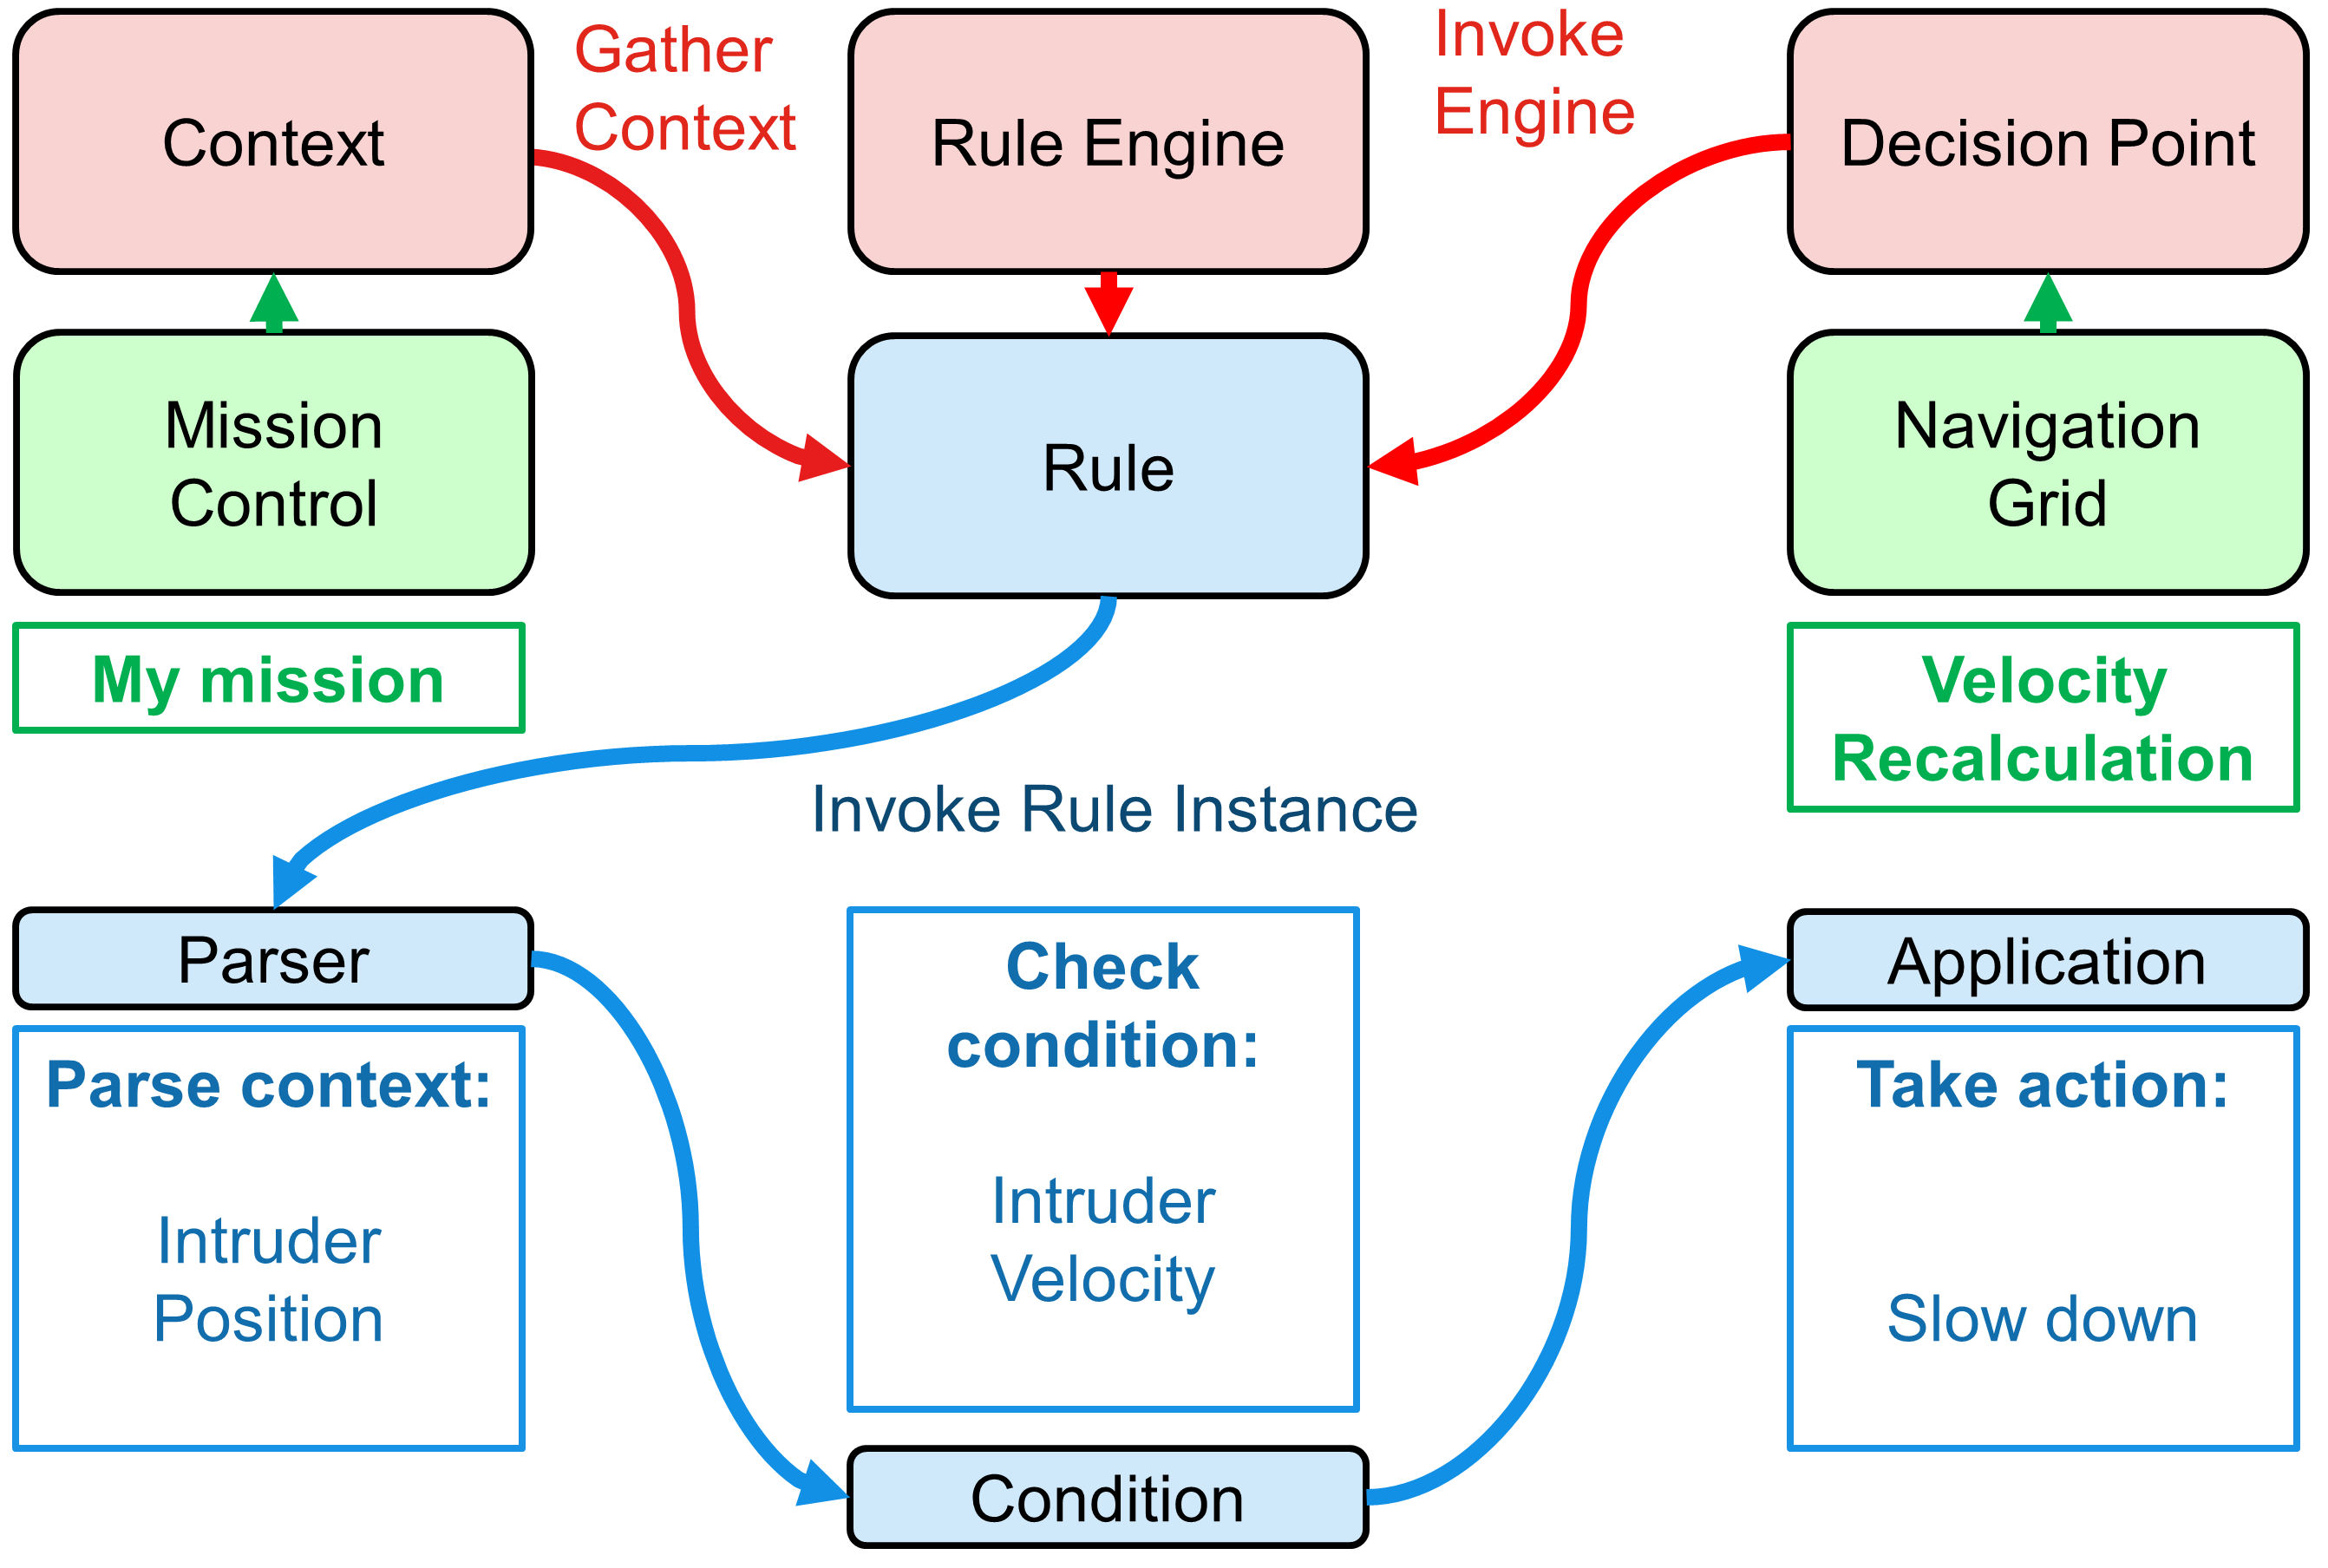
\includegraphics[width=0.7\linewidth]{\FIGDIR/RE013RuleEngineBasicArchitecture}
        \caption{Rule engine components overview.}
        \label{fig:RuleEngineBasicArchitecture}
    \end{figure}